\documentclass[12pt, twoside,a4paper, landscape]{article}
\oddsidemargin = 10pt
\textwidth = 430pt

\usepackage{fullpage}	 %to make smaller margins
\usepackage{graphicx}
%\usepackage[utf8]{inputenc}
%\usepackage[T1]{fontenc}
%\usepackage{url}

\usepackage[hidelinks]{hyperref}
\usepackage{pdfpages}
\usepackage{placeins}
\usepackage{graphicx}
\usepackage[font=small,labelfont=bf]{caption}
\usepackage{subfig}

%\usepackage{subcaption}
\usepackage{enumerate}
\usepackage{amsmath}
\usepackage{listings} %for showing program code
\usepackage{bm}
\usepackage{wrapfig}
\usepackage{lipsum}
\usepackage{float}
\usepackage{titlesec}	
\usepackage{amsfonts}
\usepackage{amssymb}
\usepackage[comma,authoryear]{natbib}
\usepackage{epstopdf}
\usepackage{array}
\usepackage{blindtext}

%\titlespacing*{\chapter}{0pt}{-10pt}{20pt}
%\titleformat{\chapter}[display]{\normalfont\huge\bfseries}{}{35pt}{}

\setlength{\intextsep}{0pt} %to make wrapfigures beautiful
%\setlength{\oddsidemargin}{0.5cm}
%\setlength{\evensidemargin}{-0.5cm}
\begin{document}
\pagenumbering{gobble}
\begin{table}[ht]
\centering
\begin{tabular}{p{0.1\textwidth}*{3}{m{0.2\textwidth}}}
Dipole&
\begin{center}Simulated on CPU\end{center}& \begin{center}Vertex shaded on GPU\end{center} &  \begin{center} Pixel shaded on GPU \end{center}
 \\
\hline
Jensen's dipole&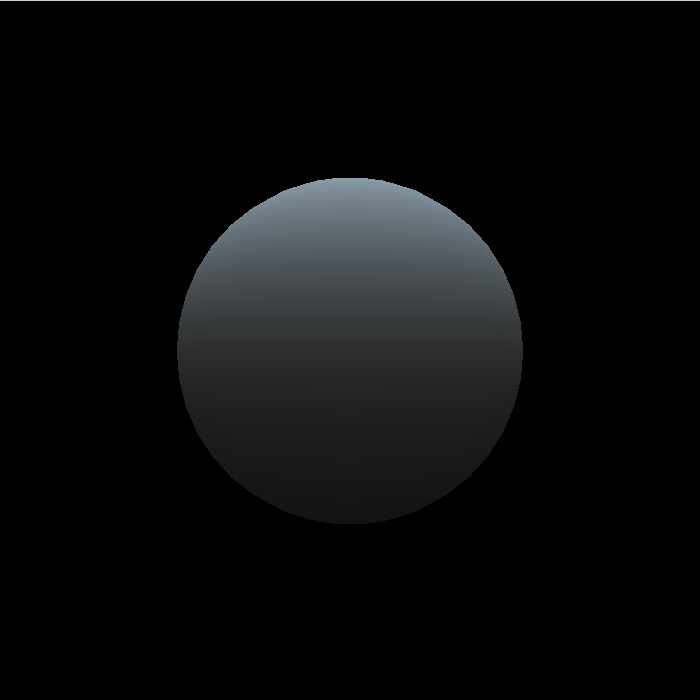
\includegraphics[scale=0.3]{jensen_simul}&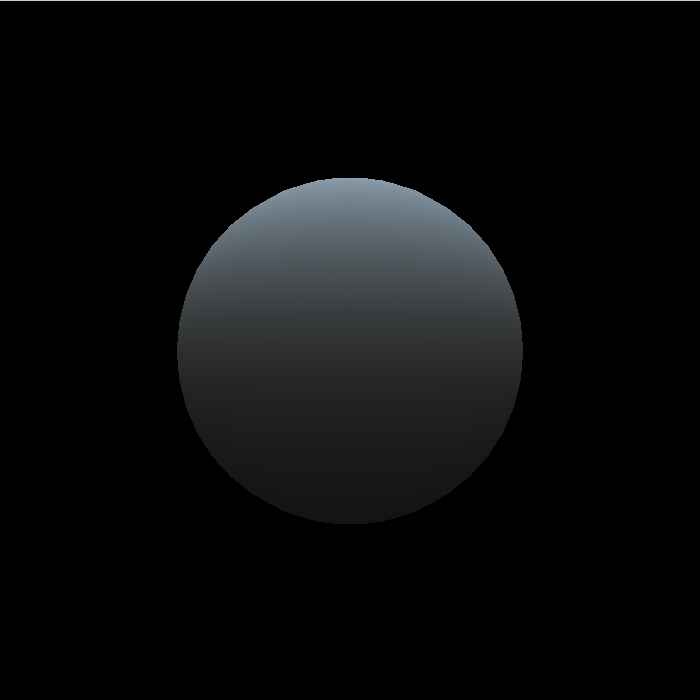
\includegraphics[scale=0.3]{jensen_vertex}&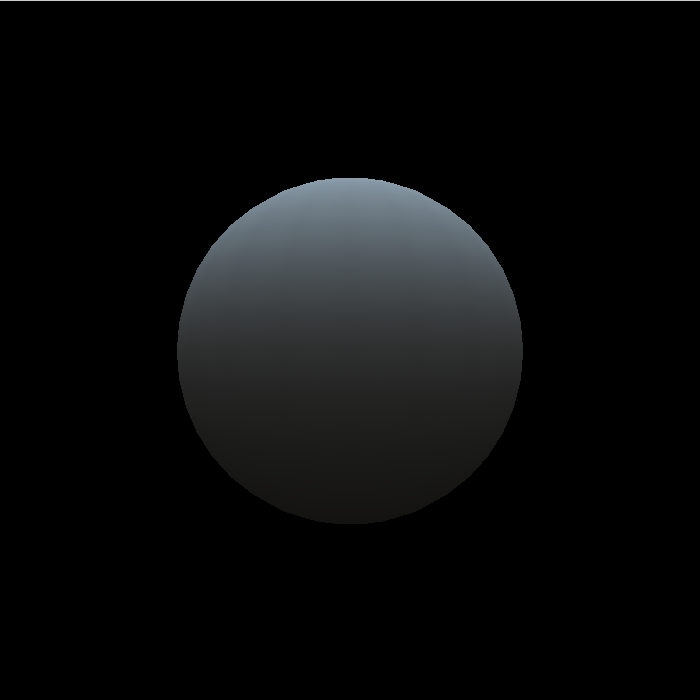
\includegraphics[scale=0.3]{jensen_pixel}\\
\hline
Better dipole&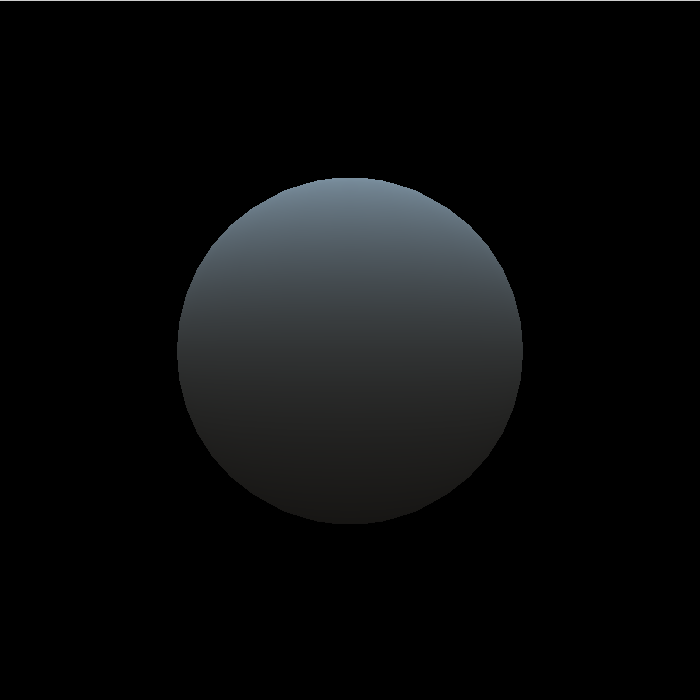
\includegraphics[scale=0.3]{deon_simul}&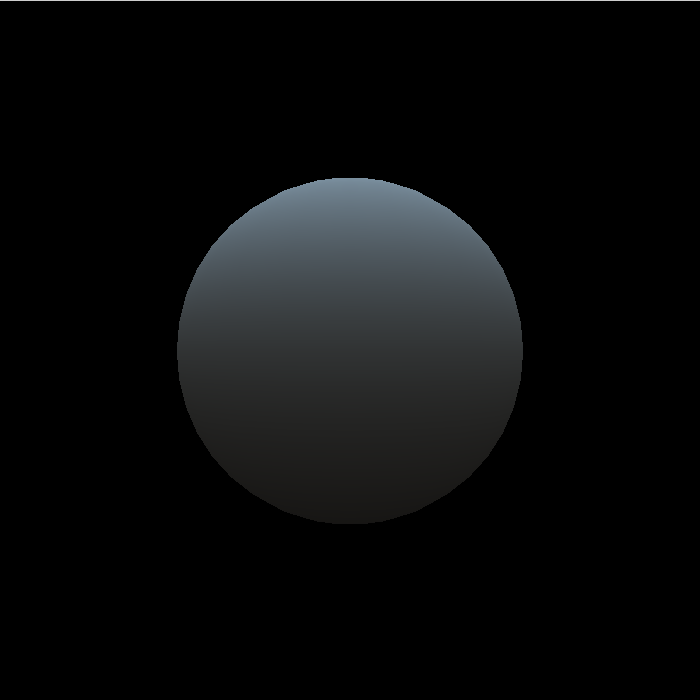
\includegraphics[scale=0.3]{deon_vertex}&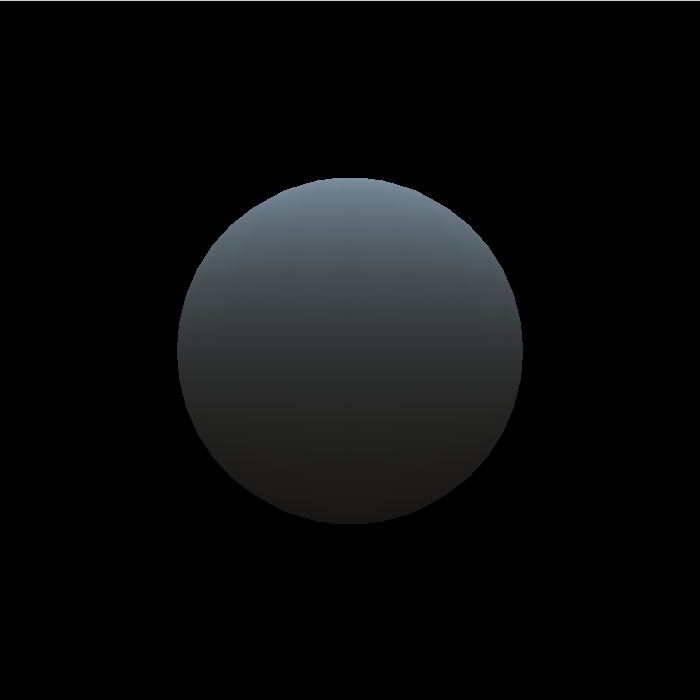
\includegraphics[scale=0.3]{deon_pixel}\\
\hline
Directional dipole&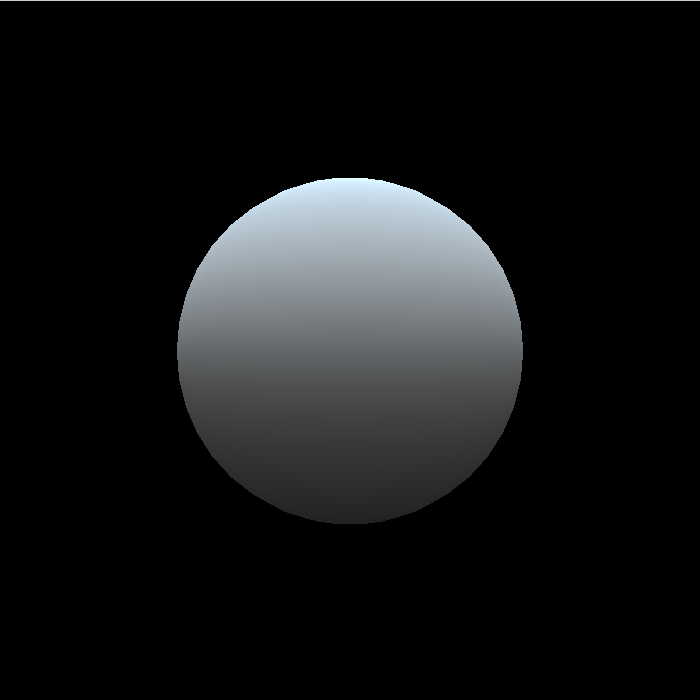
\includegraphics[scale=0.3]{jeppe_simul}&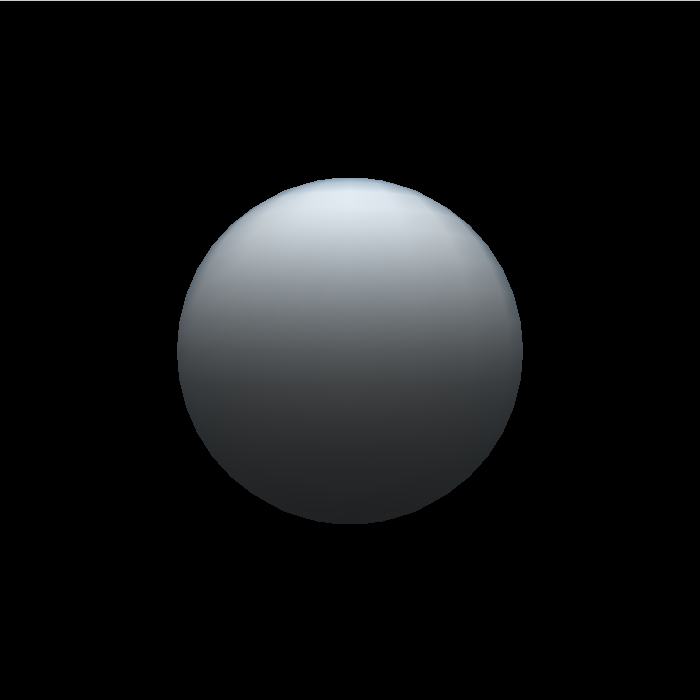
\includegraphics[scale=0.3]{jeppe_vertex}&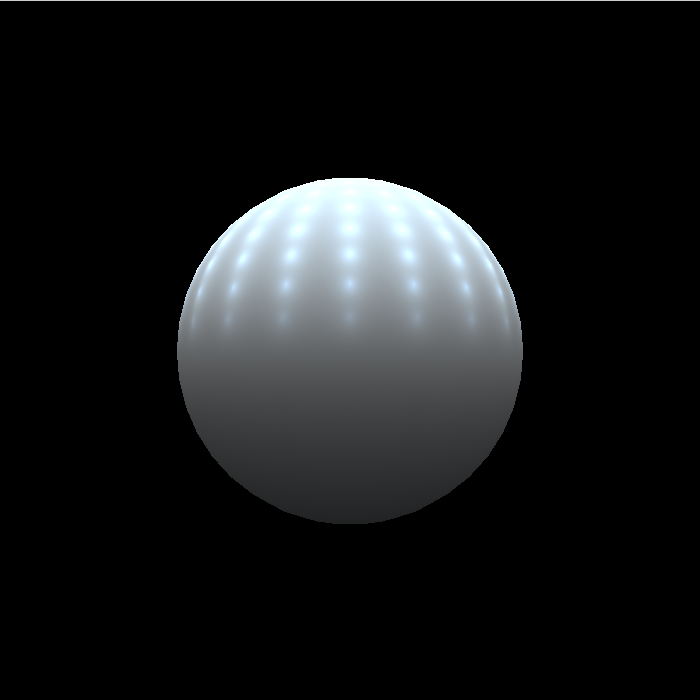
\includegraphics[scale=0.3]{jeppe_pixel}\\
\hline
\end{tabular}
\label{tab:gt}
\end{table}

\clearpage

\begin{table}[ht]
\centering
\begin{tabular}{p{0.1\textwidth}*{3}{m{0.2\textwidth}}}
Dipole&
\begin{center}Simulated on CPU\end{center}& \begin{center}Vertex shaded on GPU\end{center} &  \begin{center} Pixel shaded on GPU \end{center}
 \\
\hline
Jensen's dipole&
\includegraphics[scale=0.3]{jensen_simul_cube}&
\includegraphics[scale=0.3]{jensen_vertex_cube}&
\includegraphics[scale=0.3]{jensen_pixel_cube}\\
\hline
Better dipole&
\includegraphics[scale=0.3]{deon_simul_cube}&
\includegraphics[scale=0.3]{deon_vertex_cube}&
\includegraphics[scale=0.3]{deon_pixel_cube}\\
\hline
Directional dipole&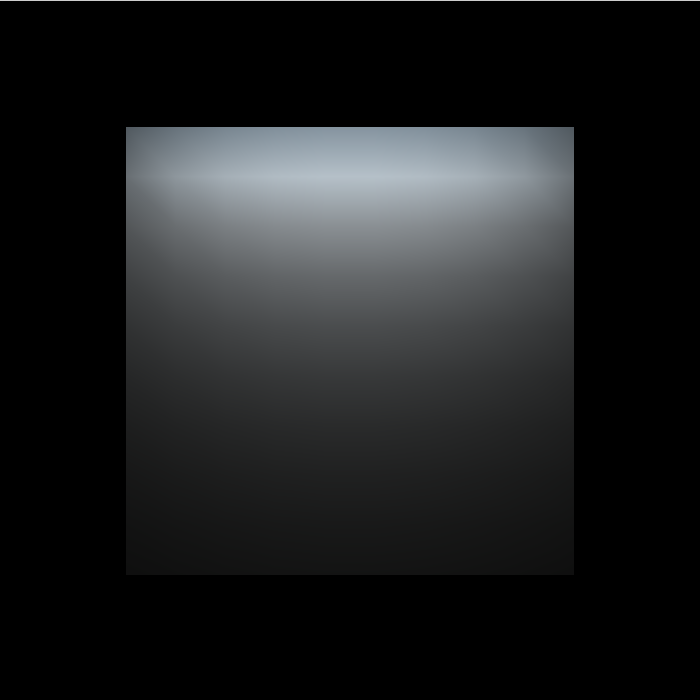
\includegraphics[scale=0.3]{jeppe_simul_cube}&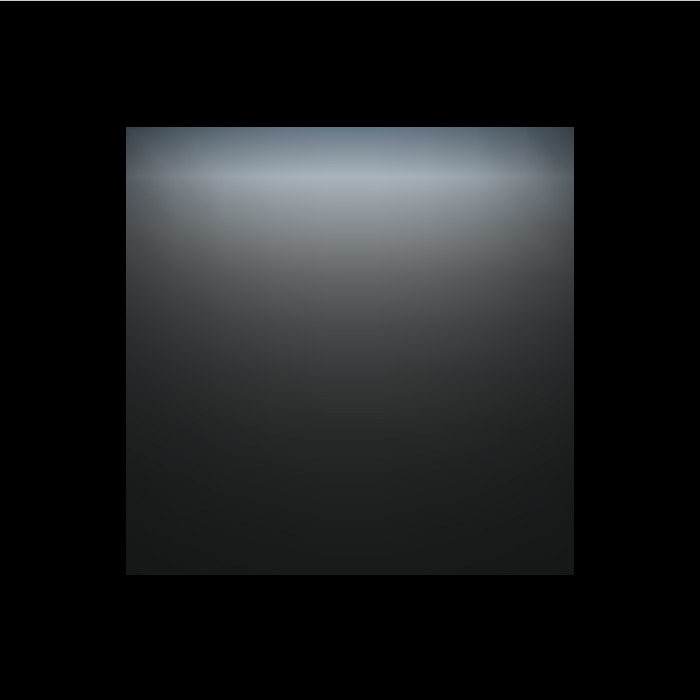
\includegraphics[scale=0.3]{jeppe_vertex_cube}&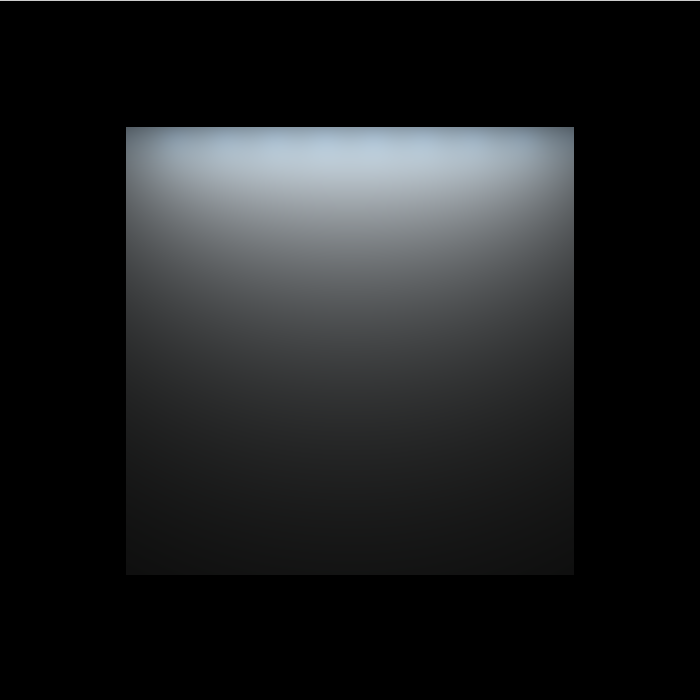
\includegraphics[scale=0.3]{jeppe_pixel_cube}\\
\hline
\end{tabular}
\label{tab:gt}
\end{table}
\clearpage
\begin{table}[ht]
\centering
\begin{tabular}{p{0.1\textwidth}*{2}{m{0.2\textwidth}}}
Dipole&
\begin{center}Vertex shaded on GPU\end{center} &  \begin{center} Pixel shaded on GPU \end{center}
 \\
\hline
Jensen's dipole&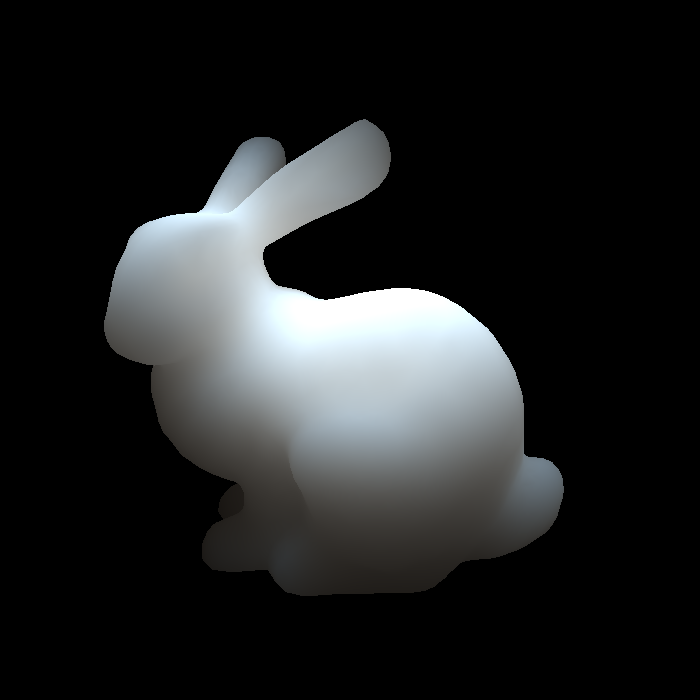
\includegraphics[scale=0.3]{jensen_vertex_bunny}&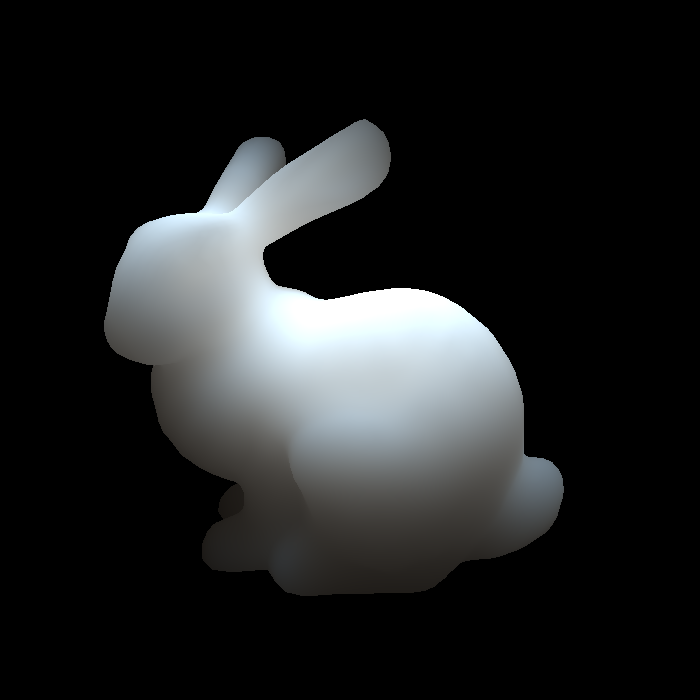
\includegraphics[scale=0.3]{jensen_pixel_bunny}\\
\hline
Better dipole&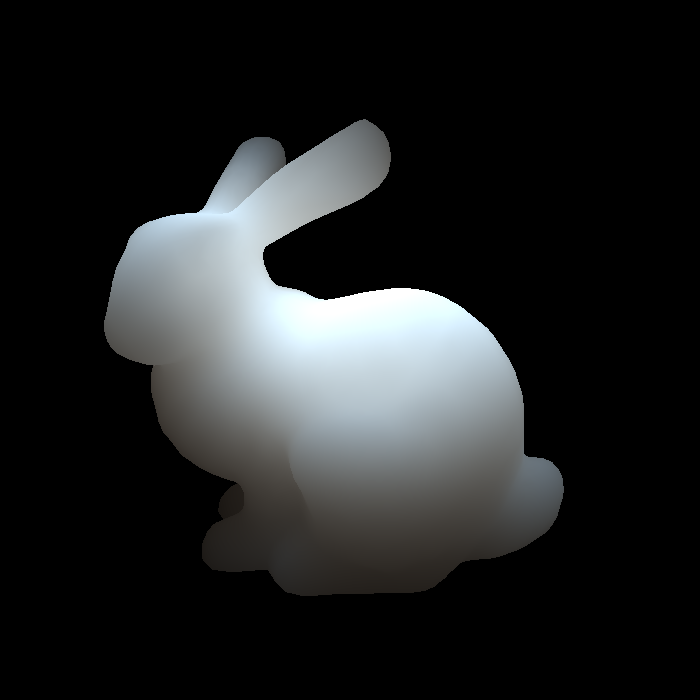
\includegraphics[scale=0.3]{deon_vertex_bunny}&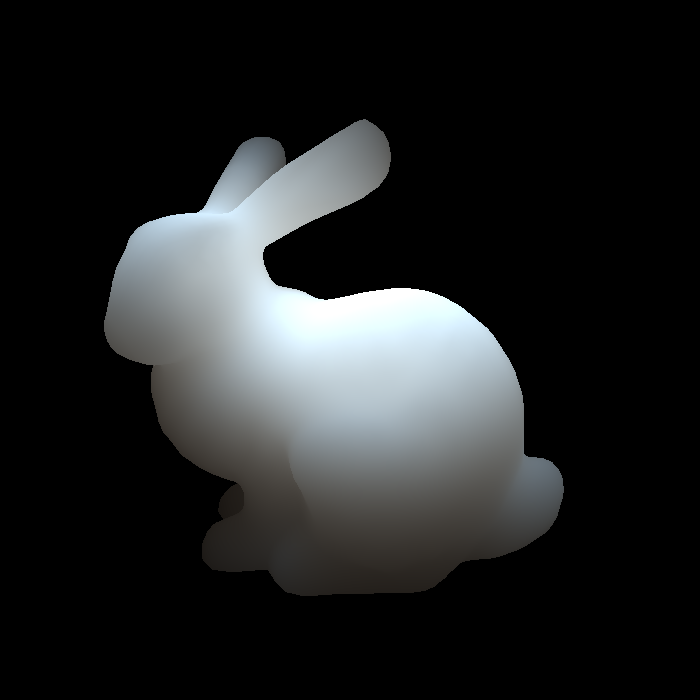
\includegraphics[scale=0.3]{deon_pixel_bunny}\\
\hline
Directional dipole&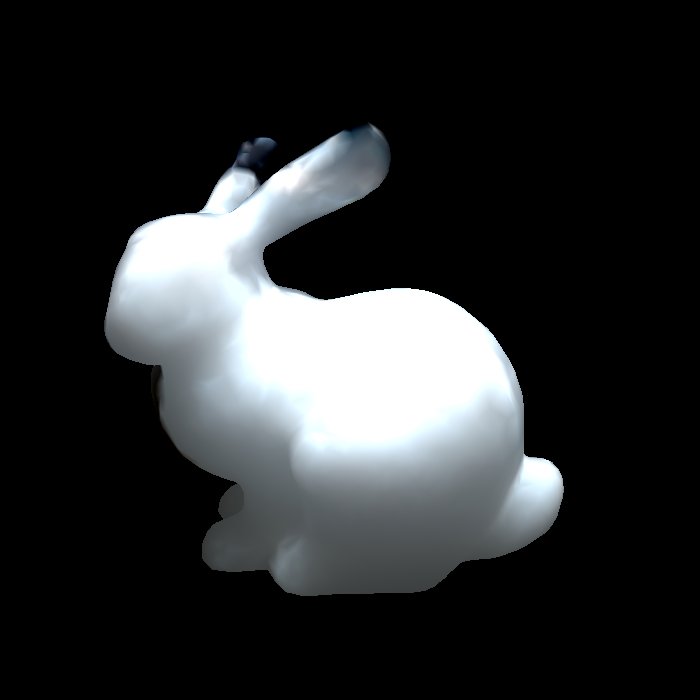
\includegraphics[scale=0.3]{jeppe_vertex_bunny}&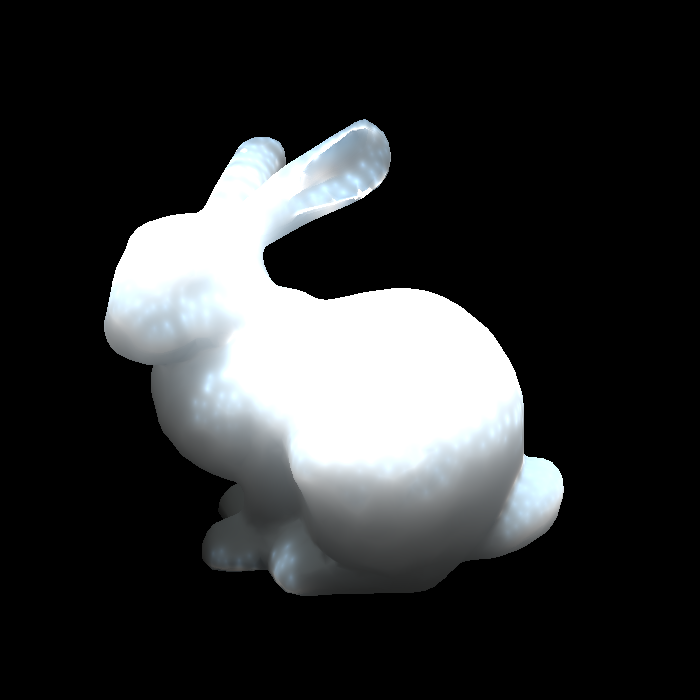
\includegraphics[scale=0.3]{jeppe_pixel_bunny}\\
\hline
\end{tabular}
\label{tab:gt}
\end{table}
\clearpage
\begin{figure}[here]
\centering
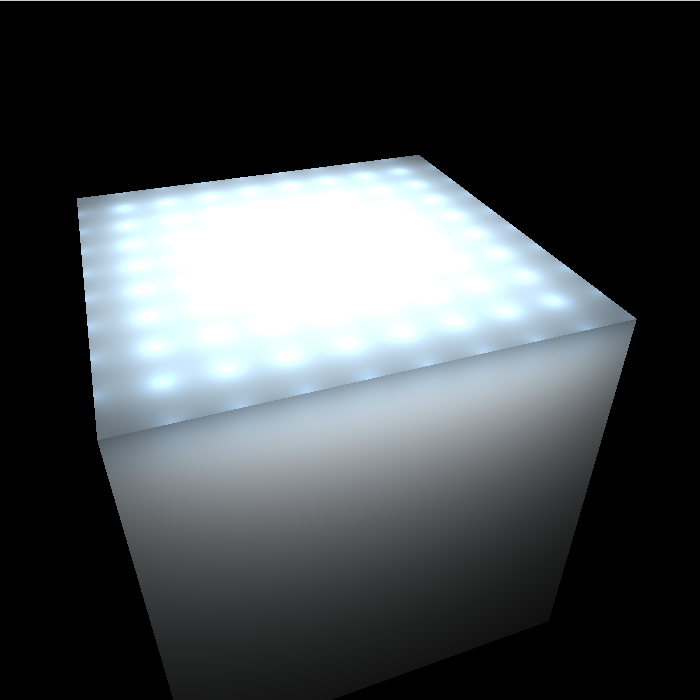
\includegraphics[width=0.4\textwidth]{artifacts}
\caption{Artifacts on directional dipole pixel shading of a cube due to undersampling.}
\end{figure}

\begin{figure}[here]
\centering
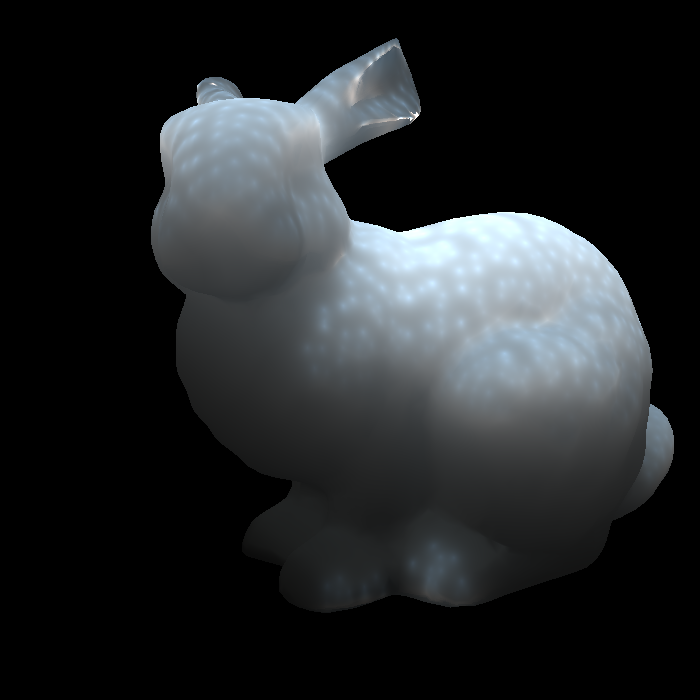
\includegraphics[width=0.4\textwidth]{artifacts_bunny}
\caption{Artifacts on directional dipole pixel shading of a bunny due to undersampling.}
\end{figure}
\end{document}
